\begin{table}[h]
    \centering
    \caption{Comparação do Tempo do Shell Sort}
    \begin{tabular}{|c|c|c|c|c|c|c|}
        \hline
        Tamanho de Entrada & 10 & 100 & 1000 & 10000 & 100000 & 1000000 \\
        \hline
        Crescente & 0.000000 & 0.000000 & 0.000000 & 0.000000 & 0.004000 & 0.063000 \\
        \hline
        Decrescente & 0.000000 & 0.000000 & 0.000000 & 0.001000 & 0.007000 & 0.083000 \\
        \hline
        Aleatória & 0.000000 & 0.000000 & 0.000000 & 0.001000 & 0.022000 & 0.300000 \\
        \hline
    \end{tabular}
    \label{tab:comparacaoshell}
\end{table}

A Tabela \ref{tab:comparacaoshell} mostra o Bubble Sort nos 6 diferentes tamanhos
de entrada e 3 situações diferentes de como as entradas são postas em determinados arquivos. Os resultados mostram que o algoritmo executa muito rápido até para entradas muito grande. Diferentemente dos algoritmos de ordenação mais simples, como Bubble Sort e Selection Sort, o Shell Sort emprega uma estratégia de redução de intervalo para melhorar a eficiência do Insertion Sort, conseguindo assim lidar com conjuntos de dados mais amplos de maneira mais eficaz. Mesmo na forma aleatória ter sido maior que as demais com muitas entradas, é um valor insignificante pois não passa de um segundo de execução.

\begin{figure}[h!]
    \centering
    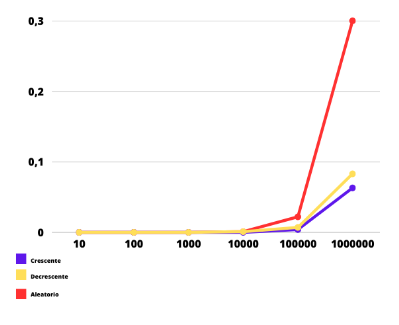
\includegraphics[width = 10cm]{Imagens/Shell Sort/Captura de tela 2023-09-27 211633.png}
    \caption{Gráfico de tempo do algoritmo Shell Sort.}
    \label{fig:shell1}
\end{figure}